% ============================================================
%  SECTION 7 (was C): The RBI and India's reserves  (Member 3)
%  Member 3's text. Changes at merge:
%   - Did you know box now uses RBI (2026) and World Bank figures instead of
%     Wikipedia/Deccan Chronicle; "about two weeks of imports" used book-wide
%   - reserves chart redrawn from the full annual World Bank series (1990-2025)
%   - new figure showing intervention in the demand-and-supply diagram
% ============================================================
\section{The RBI and India's foreign exchange reserves}\label{sec:reserves}

We have seen how the RBI intervenes in the foreign exchange market to stabilise the rupee. But what exactly does it intervene with? The answer lies in India's \keyterm{foreign exchange reserves}{Foreign currency assets, gold and other reserve assets held by the RBI on behalf of the country.}, a stockpile of assets that the RBI holds and manages on behalf of the country.

India's foreign exchange reserves are made up of four components. The largest part is \textbf{foreign currency assets}, holdings of major currencies like the US dollar, euro and pound sterling, typically invested in safe foreign government securities. The second component is \textbf{gold}. The third is \keyterm{Special Drawing Rights (SDR)}{An international reserve asset created by the IMF that member countries can use to settle payments with each other.}, an international reserve asset created by the IMF that member countries can use to settle payments with other nations. The fourth is India's \textbf{reserve position with the IMF}, the amount India can draw on demand without conditions.

Why does a country hold these reserves? There are three main reasons. First, they act as a buffer against economic shocks: if exports collapse or a financial panic hits, reserves can cushion the blow. Second, they ensure the country can pay for its imports even during difficult times. A commonly used measure is \keyterm{import cover}{The number of months of imports a country could pay for using only its reserves.}, which tells us how many months of imports a country could pay for using only its reserves. Third, large reserves signal financial stability to foreign investors, encouraging investment.

\begin{didyouknow}{From crisis to confidence}
In mid-1991, India's foreign exchange reserves could pay for only about two weeks of imports. On 29 May 2026 they stood at US\$682 billion, enough for about 11 months of imports (Reserve Bank of India [RBI], 2026c). Measured at the end of each year, they grew from US\$5.6 billion in 1990 to US\$700 billion in 2025, a rise of more than 120 times in 35 years (World Bank, 2026b).
\end{didyouknow}

Figure~\ref{fig:reserves} shows how India's foreign exchange reserves have grown since 1990.

\begin{figure}[!htb]
  \centering
  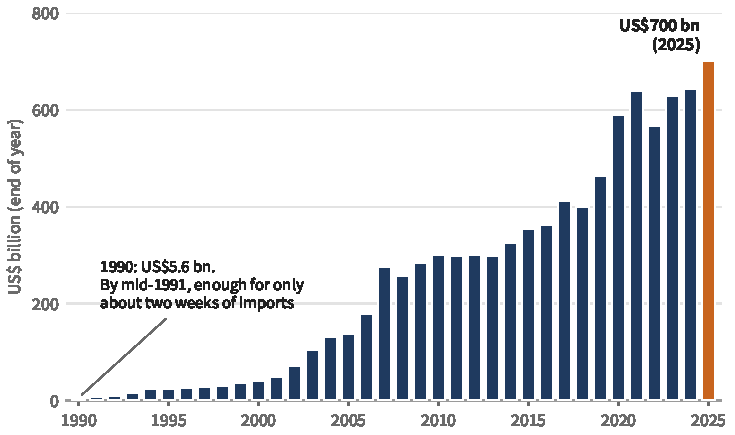
\includegraphics[width=\linewidth]{figures/reserves.pdf}
  \caption{India's foreign exchange reserves, 1990--2025 (US\$ billion, end of year).}
  \label{fig:reserves}
  {\raggedright\small\sffamily Reserves include foreign currency assets, gold, SDRs and the reserve position with the IMF. Notice the dips in 2008 and 2022, partly because the RBI sold dollars to steady the rupee \seesec{sec:moves}.\par}
  \figsource{World Bank (2026b), World Development Indicators, series FI.RES.TOTL.CD.}
\end{figure}

Now let us look at how the RBI uses these reserves to manage the rupee's value. Suppose the rupee is falling too fast against the US dollar, perhaps because too many people are selling rupees to buy dollars. The RBI steps in by selling dollars from its reserves into the foreign exchange market. This \keyterm{intervention}{Buying or selling foreign currency by the central bank to influence the exchange rate.} increases the supply of dollars, making the dollar relatively cheaper and the rupee relatively more valuable, slowing or reversing the rupee's fall (Figure~\ref{fig:intervene}). The opposite happens when the rupee is rising too fast: the RBI buys dollars, increasing demand for the dollar and gently pushing the rupee's value back down.

\begin{figure}[!htb]
  \centering
  % Figure (Section 7, new at merge): how RBI intervention slows a fall in the rupee.
% Demand shifts right by 1 (A ₹85 -> B ₹90); the RBI sells dollars, supply shifts
% right by 0.6 (-> C ₹87). Same geometry as Figures 4 and 10.
\begin{tikzpicture}[ds, x=1.1cm, y=1.1cm]
\draw[ds axis] (0,0) -- (0,3.7) node[above] {₹ per US dollar};
\draw[ds axis] (0,0) -- (5,0);
\node[below] at (2.5,0) {Quantity of US dollars};
\draw[ds demand] (0.4,3.2) -- (3.6,0.6) node[below] {D\textsubscript{0}};
\draw[ds demand, ds new] (1.4,3.2) -- (4.6,0.6) node[below] {D\textsubscript{1}};
\draw[ds supply] (0.4,0.6) -- (3.6,3.2) node[above] {S\textsubscript{0}};
\draw[ds supply, draw=fxteal] (1.0,0.6) -- (4.2,3.2) node[above right=-2pt, text=fxteal, align=left] {S\textsubscript{1}: RBI\\sells dollars};
\draw[ds guide] (0,1.9) -- (2,1.9) -- (2,0);
\draw[ds guide] (0,2.306) -- (2.5,2.306);
\draw[ds guide] (0,2.062) -- (2.8,2.062) -- (2.8,0);
\draw[ds shift] (2.95,1.2) -- (3.75,1.2);
\draw[ds shift, fxteal] (3.12,2.75) -- (3.58,2.75);
\node[ds eq] at (2,1.9) {}; \node[below=3pt] at (2,1.9) {A};
\node[ds eq=fxorange] at (2.5,2.306) {}; \node[above=3pt, text=fxorange] at (2.5,2.306) {\textbf{B}};
\node[ds eq=fxteal] at (2.8,2.062) {}; \node[below right=1pt, text=fxteal] at (2.8,2.062) {\textbf{C}};
\node[left] at (0,1.86) {85};
\node[left, text=fxteal] at (0,2.08) {\textbf{87}};
\node[left, text=fxorange] at (0,2.33) {\textbf{90}};
\end{tikzpicture}

  \caption{How RBI intervention slows a fall in the rupee (hypothetical numbers).}
  \label{fig:intervene}
  {\raggedright\small\sffamily 1. The market starts at A, ₹85 per US dollar. 2. A bigger oil bill shifts demand for dollars right to D\textsubscript{1}. Left alone, the rate would rise to ₹90 at B. 3. The RBI sells dollars from its reserves, so supply shifts right to S\textsubscript{1}. 4. The market settles at C, ₹87: the rupee still falls, but by less, and India's reserves are smaller by the dollars the RBI sold.\par}
  \figsource{Drawn by the authors.}
\end{figure}

However, this tool has clear limits. Foreign exchange reserves, however large, are finite. If strong and sustained market pressure is pushing the rupee in one direction, the RBI cannot fight it indefinitely. This is precisely what happened in 1991, and it is a reminder that while reserves give the RBI significant power to stabilise the currency in the short run, they cannot override fundamental economic forces over the long run \seesec{sec:crises}.
